%% LaTeX Beamer presentation template (requires beamer package)
%% see http://bitbucket.org/rivanvx/beamer/wiki/Home
%% idea contributed by H. Turgut Uyar
%% template based on a template by Till Tantau
%% this template is still evolving - it might differ in future releases!

\documentclass{beamer}

\mode<presentation>
{
\usetheme{Warsaw}

\setbeamercovered{transparent}
}

\usepackage[english]{babel}
\usepackage[utf8]{inputenc}

% font definitions, try \usepackage{ae} instead of the following
% three lines if you don't like this look
\usepackage{mathptmx}
\usepackage[scaled=.90]{helvet}
\usepackage{courier}
%\usepackage{ae}


\usepackage[T1]{fontenc}

\usepackage{multicol}

\usepackage[round]{natbib}


\title{Acessibilidade nas fases de Engenharia de Requisitos, Projeto e Codificação de Software: Uma ferramenta de apoio}

\subtitle{Defesa de Dissertação de Mestrado}

% - Use the \inst{?} command only if the authors have different
%   affiliation.
%\author{F.~Author\inst{1} \and S.~Another\inst{2}}
\author{\mbox{Rodrigo G. de ~Branco} \and \mbox{Profª. Drª. Débora M. B. ~Paiva (Orientadora)}}

% - Use the \inst command only if there are several affiliations.
% - Keep it simple, no one is interested in your street address.
\institute[Universities of]
{
Faculdade de Computação\\
Universidade Federal de Mato Grosso do Sul
}

\date{09 de Setembro de 2013}


% This is only inserted into the PDF information catalog. Can be left
% out.
\subject{Talks}



% If you have a file called "university-logo-filename.xxx", where xxx
% is a graphic format that can be processed by latex or pdflatex,
% resp., then you can add a logo as follows:

\pgfdeclareimage[height=0.5cm]{university-logo}{university-logo-filename}
\logo{\pgfuseimage{university-logo}}



% Delete this, if you do not want the table of contents to pop up at
% the beginning of each subsection:
\AtBeginSubsection[]
{
\begin{frame}<beamer>
\frametitle{Roteiro}
	\begin{multicols}{2}
		\tableofcontents[currentsection,currentsubsection]
	\end{multicols}
\end{frame}
}

% If you wish to uncover everything in a step-wise fashion, uncomment
% the following command:

%\beamerdefaultoverlayspecification{<+->}

\begin{document}

\begin{frame}
\titlepage
\end{frame}

\begin{frame}
\frametitle{Roteiro}
	\begin{multicols}{2}
		\tableofcontents
	\end{multicols}
% You might wish to add the option [pausesections]
\end{frame}


\section{Introdução e Motivação} 

\subsection[Motivação]{Motivação}

\begin{frame}
\frametitle{Internet}
\framesubtitle{}

\begin{itemize}
  \item Importante meio de disseminação de informação
  \item Ferramenta essencial nas atividades cotidianas
  \item Alguns serviços disponibilizados \textbf{APENAS} por essa via \citep{irpf:13,tjce:11}
\end{itemize}

\end{frame}

\begin{frame}
\frametitle{Utilização da Internet como apoio aos negócios}
\framesubtitle{Benefícios \citep{oliveira:11}}

\begin{itemize}
  \item Disponibilidade de 24 horas por dia;
  \item Possibilidade de acesso de todas as partes do planeta - ou fora dele? \citep{curiosity:13};
  \item Necessidade de espaço físico e de infra-estrutura reduzidos (ex: bancos) para realizar;
as atividades;
  \item Custo de investimento inicial baixo, entre outros.
\end{itemize}

\end{frame}

\begin{frame}
\frametitle{Acesso equalitário à informação}
\framesubtitle{}

\begin{itemize}
  \item Acesso homogêneo aos recursos da Internet \citep{5260918}
  \item Única forma de acesso à informação por alguns grupos de usuários
  \item Pessoas diferentes com problemas diferentes, equipamentos diferentes, \textit{softwares} diferentes e necessidades diferentes
  \item Pessoas com deficiências são prejudicadas por soluções malfeitas
\end{itemize}

\end{frame}

\begin{frame}
\frametitle{Produto \textit{web} acessível}
\framesubtitle{}

\begin{itemize}
  \item É difícil garantir um produto 100\% acessível
  \item Domínio de estudo relativamente novo
  \item Várias pesquisas na área \citep{lazar:04,brajnik:06,zeng:05}
  \item Papel fundamental da Engenharia de \textit{Software} no processo de desenvolvimento
  \item Os custos são menores quando a acessibilidade é considerada durante o processo de desenvolvimento
do \textit{software} \citep{groves:11}
\end{itemize}

\end{frame}

\subsection[Problema]{Problema}

\begin{frame}[allowframebreaks]
\frametitle{Observações}
\framesubtitle{}

\begin{itemize}
  \item Integração de tópicos de Acessibilidade no processo de desenvolvimento \citep{springerlink:10.1007/978-3-642-02713-0,maia:10}
  \item Rastreabilidade dos requisitos de acessibilidade
  \item Muitos desenvolvedores não sabem como codificar de forma a tornar seus produtos acessíveis \citep{1630123,alves:11}
  \item Desenvolvedores não estão satisfeitos com as ferramentas de apoio à acessibilidade disponíveis \citep{Trewin:2010:ACT:1805986.1806029}
  \item Desenvolvedores estão insatisfeitos em utilizar ferramentas externas ao
seu ambiente de desenvolvimento para efetuar a avaliação \citep{Trewin:2010:ACT:1805986.1806029}
  \item As ferramentas nem sempre informam de forma objetiva as mudanças necessárias para fornecer um produto acessível \citep{groves:12}
  \item A avaliação normalmente ocorre quando o produto já está pronto (Refatoramento)  
\end{itemize}

\end{frame}

\subsection[Objetivos]{Objetivos}

\begin{frame}
\frametitle{Objetivos gerais}
\framesubtitle{}

\begin{itemize}
 \item Estender o MTA, propondo uma metologia para a rastreabilidade dos requisitos de acessibilidade atravées do processo de desenvolvimento de \textit{software}
 \item Permitir a associação explícita entre os requisitos de acessibilidade e os artefatos de documentação e, para cada associação, especificar uma ou mais técnicas de implementação de acessibilidade de acordo com o documento de conformidade em acessibilidade escolhido
 \item Implementar uma ferramenta de suporte que seja integrada ao ambiente de desenvolvimento e que implemente os objetivos listados acima
\end{itemize}

\end{frame}

\begin{frame}[allowframebreaks]
\frametitle{Características desejáveis para a ferramenta}
\framesubtitle{Partindo da pesquisa de \citet{Trewin:2010:ACT:1805986.1806029}}

\begin{itemize}
 \item Seja orientada ao desenvolvedor (a apresentação dos resultados nas ferramentas tradicionais são adequadas para avaliação e auditoria de sites, e não para desenvolvedores)
 \item Seja integrada ao ambiente de desenvolvimento do desenvolvedor
 \item Apresente informações objetivas e no momento em que o desenvolvedor desejar visualizar
 \item Tenha relação direta entre os requisitos e casos de uso com a etapa de codificação
 \item Permita que seja feita o rastreamento dos requisitos de acessibilidade, desde a sua concepção até as fases de codicação
 \item Permita que o desenvolvedor consiga verificar, em nível de código, a associação dos requisitos e modelos
\end{itemize}

\end{frame}

\subsection[Metodologia]{Metodologia}

\begin{frame}[allowframebreaks]
\frametitle{Passos necessários para atingir aos objetivos}
\framesubtitle{}

\begin{itemize}
 \item Estudar a literatura sobre o assunto
 \item Identificar os pontos de integração entre as atividades de engenharia de requisitos, projeto e geração de cóodigo
 \item Estudar o processo de desenvolvimento de plugins para o Eclipse
 \item Estudar como técnicas de acessibilidade podem ser associadas aos modelos
 \item Estudar quais tecnologias existentes podem ser usadas para efetuar a associação dos requisitos e modelos às téecnicas de acessibilidade
 \item Desenvolver a ferramenta
 \item Efetuar uma prova de conceito, criando um projeto utilizando o MTA e a ferramenta proposta
\end{itemize}

\end{frame}

\section{Fundamentação Teórica}
 
\subsection[Acessibilidade na Web]{Acessibilidade na Web}

\begin{frame}
\frametitle{Contextualização}
\framesubtitle{}

\begin{itemize}
 \item A Internet foi projetada para para ser usada sem \textit{mouse}, até sem os olhos \citep{thatcher:06}
 \item Tecnologias como \textit{Javascript} e \textit{Flash} deixaram a Internet mais atrativa, mas\ldots
 \pause
 \item o uso indiscriminado dessas tecnologias podem, ao mesmo tempo, facilitar, inibir ou impedir o acesso aos recursos
 \item Desafio: Conscientização dos desenvolvedores \citep{freire:08,alves:11}
\end{itemize}

\end{frame}

\begin{frame}
\frametitle{Tecnologias Assistivas}
\framesubtitle{}

\begin{itemize}
  \item Conjunto de equipamentos, serviços, estratégias e práticas concebidas para atenuar os problemas encontrados pelas pessoas com necessidades especiais \citep{cook:95}
  \item Cegueira
  \item Baixa visão
  \item Deficiência física
  \item Deficiência auditiva
\end{itemize}

\end{frame}

\begin{frame}
\frametitle{Legislação}
\framesubtitle{}

\begin{itemize}
  \item Começou com a \textit{Section 508} (USA), em 1998 \citep{section508:98}
\end{itemize}

\begin{itemize}
  \item Posteriormente\ldots
  \begin{itemize}
    \item DDA (UK) \citep{dda:95}
    \item Leis 10.048/2000 e 10.098/2000 (BR)
    \item entre outros\ldots
   \end{itemize}
\end{itemize}

\end{frame}

\begin{frame}
\frametitle{Documentos e padrões}
\framesubtitle{W3C e WAI}

\begin{figure}[htbp] \centering
	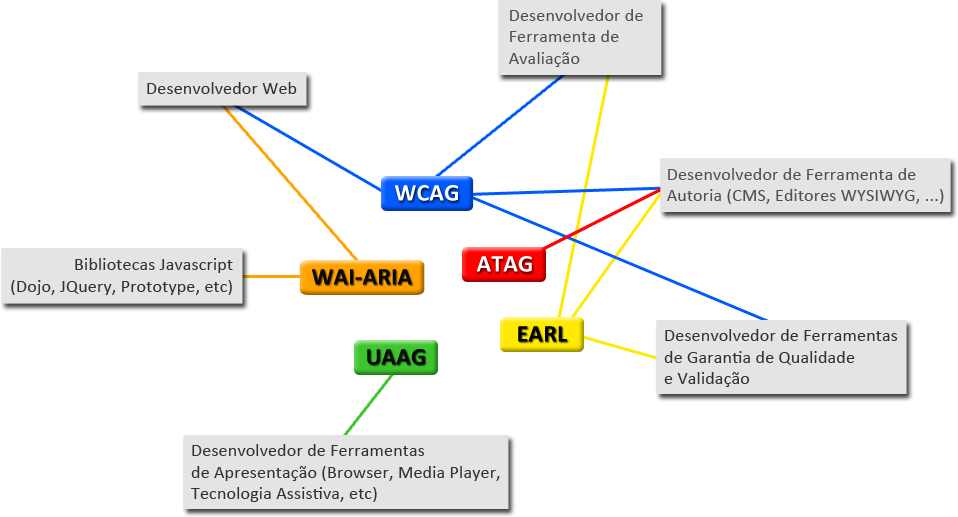
\includegraphics[width=\textwidth]{./img/relation.jpg}
	\caption{Documentos e relação com os desenvolvedores}
	\label{fig:sub4}
\end{figure}

\end{frame}

\begin{frame}
\frametitle{Documentos e padrões}
\framesubtitle{Breve descrição}

\begin{itemize}
  \item WCAG (1.0 e 2.0): Documento de referência com diretrizes e recomendações para implementação de acessibilidade
  \item WAI-ARIA (1.0 - candidata): define como a funcionalidade do elemento deve ser entregue à tecnologia assistiva
  \item ATAG (1.0 e 2.0 - rascunho): destinado aos desenvolvedores de ferramentas de autoria, para que o conteúdo gerado por estas ferramentas seja acessível
  \item UAAG (1.0 e 2.0 - rascunho): destinado aos desenvolvedore de \textit{User Agents}
  \item EARL (1.0 - rascunho): formato definido para expressar resultados de testes, principalmente por ferramentas de avaliação automática 
\end{itemize}

\end{frame}

\begin{frame}
\frametitle{WCAG 2.0}
\framesubtitle{}

\begin{itemize}
  \item Documento de referência
  \item Fornece abordagens, técnicas, critérios de sucesso e testes
  \item 3 níveis de prioridade (A, AA, AAA)
  \item 14 diretrizes
  \item Vários documentos derivados
  \begin{itemize}
   	\item CLF (CA) \citep{clf:13}
   	\item NDA (IE) \citep{nda:13}
   	\item eMag (BR) \citep{emag:13}
   	\item Diretrizes de \textit{design} da Microsoft \citep{microsoft:11}   	
   \end{itemize}
\end{itemize}

\end{frame}

\subsection[Pesquisa Bibliográfica]{Pesquisa Bibliográfica}

\begin{frame}
\frametitle{Acessibilidade no contexto de Engenharia de \textit{Software}}
\framesubtitle{Divisão das áreas de interesse}

\begin{itemize}
  \item Requisitos
  \item Arquitetura
  \item Navegação
  \item Interface
  \item Conteúdo
  \item Avaliação
  \item Processo de Desenvolvimento
\end{itemize}

\end{frame}

\begin{frame}
\frametitle{Principais artigos}
\framesubtitle{Requisitos - \citet{Trewin:2010:ACT:1805986.1806029}}

\begin{itemize}
  \item Pesquisa com desenvolvedores da IBM
  \item \textit{Status} das ferramentas de apoio à acessibilidade
  \item \textit{Design}, testes e identificação de soluções tecnológicas é uma tarefa difícil
  \item Os desenvolvedores não confiam nas informações fornecidas pela ferramenta
  \item As informações fornecidas pelas ferramentas nem sempre são claras e objetivas
  \item As ferramentas não são integradas ao ambiente de desenvolvimento
\end{itemize}

\end{frame}

\begin{frame}
\frametitle{Principais artigos}
\framesubtitle{Requisitos - \citet{analuizadias:2010}}

\begin{itemize}
  \item Inserção de acessibilidade nas etapas de desenvolvimento de \textit{software}
  \item Pesquisa nos principais portais (Springer, ACM, IEEE, Elsevier, Wiley e Scielo)
  \item Muitas pesquisas referentes a testes com usuários
  \item Nenhuma com instalação de \textit{software}
\end{itemize}

\end{frame}

\begin{frame}
\frametitle{Principais artigos}
\framesubtitle{Arquitetura - \citet{Fuertes:2011:DHW:1969289.1969294}}

\begin{itemize}
  \item \textit{Hera-FFX} - Hera (WCAG 2.0) para Firefox
  \item Características desejáveis de uma ferramenta de avaliação:
  	\begin{multicols}{2}
  	\begin{itemize}
  	 	\item Avaliação preliminar automática
  	 	\item Suporte para preenchimento manual
  	 	\item Modicação da página de apresentação
  	 	\item Exibição do código anotado
  	 	\item Avaliação de páginas locais
  	 	\item Avaliação de páginas com acesso restrito
  	 	\item Avaliação de renderização de páginas
  	 	\item Geração de relatórios
  	 	\item Suporte para treinamento
  	 	\item Capacidade de multi-sessão
  	 	\item Flexibilidade
  	 \end{itemize}
  	\end{multicols}
\end{itemize}

\end{frame}

\begin{frame}
\frametitle{Principais artigos}
\framesubtitle{Interface - \citet{Halbach:2010:TCA:1747589.1747607}}

\begin{itemize}
  \item Deficiência cognitiva
  \item WCAG cobre uma área limitada dessas deficiências
  \item O autor propôs um conjunto de princípios de \textit{design} para cada sub-área
  \item Padrões de design pouco usuais em desenvolvimento de sites
\end{itemize}

\end{frame}

\begin{frame}
\frametitle{Principais artigos}
\framesubtitle{Avaliação - \citet{Vigo:2011:AWA:1963660.1963798}}

\begin{itemize}
  \item Métricas de acessibilidade
  \item Qual é a ``qualidade'' das métricas existentes
  \item Algumas métricas são difíceis de implementar e testar
  \item Melhores métricas para o quesito \textit{validez}: WAQM, PM e WAB
  \item PM não teve um bom desempenho para o quesito \textit{adequação}
\end{itemize}

\end{frame}

\begin{frame}
\frametitle{Principais artigos}
\framesubtitle{Avaliação - \citet{Brajnik:2009:VRW:1639642.1639666}}

\begin{itemize}
  \item Validade das diretrizes de acessibilidade (WCAG 1.0 e 2.0)
  \item Um mesmo conjunto de diretrizes de acessibilidade produzirá os mesmos resultados, se conduzido por pessoas ou ferramentas diferentes?
  \item Se sim, qual é a qualidade dos métodos de avaliação utilizados e o quão ``testáveis'' são as diretrizes de acessibilidade
  \item O autor concluiu que:
  \begin{itemize}
    \item As diretrizes doWCAG 1.0 são mais confiáveis do que as diretrizes do WCAG 2.0
    \item O nível de confiabilidade das diretrizes nãoo pode ser considerado alto, já que este nível não ultrapassou 80\%
  \end{itemize}
\end{itemize}

\end{frame}

\begin{frame}[allowframebreaks]
\frametitle{Principais artigos}
\framesubtitle{Avaliação - \citet{freire:12}}

\begin{itemize}
  \item Estudo com grupos específicos de usuários com deficiência
  \item Quais são as características principais dos problemas de acessibilidade encontrados?
  \item Qual a relação entre utilizar uma medição de acessibilidade utilizando uma abordagem
baseada no usuário e uma medição técnica baseada nas diretrizes do WCAG 1.0 e 2.0?
  \item O autor concluiu que:
  \begin{itemize}
   	\item Os sites possuem variados níveis de barreiras, dependendo da deficiência que o usuário possui
   	\item Não há uma correlação significativa entre as classificações das gravidades de problemas de usuários e os níveis de prioridades associadas aos \textit{checkpoints} e critérios de sucesso do WCAG 1.0
   	\item Sites com altos níveis de conformidade técnica não implicam em sites isentos de problemas encontrados pelo usuário
  \end{itemize}
\end{itemize}

\end{frame}


\subsection[MTA]{Acessibilidade no Processo de Desenvolvimento}

\begin{frame}
\frametitle{MTA - \citet{maia:10}}
\framesubtitle{}

\begin{itemize}
  \item Extensão da ISO/IEC 12207 (Processo de Desenvolvimento)
  \item Tem como objetivo guiar o processo de desenvolvimento desde as fases iniciais para que a aplicação que está sendo desenvolvida seja acessível
  \item Inclusão de Tarefas de acessibilidade nos subprocessos:
  	\begin{multicols}{2}
  	\begin{itemize}
  	 	\item Elicitação dos requisitos do sistema
  	 	\item Análise dos requisitos do sistema
  	 	\item Projeto Arquitetural do sistema
  	 	\item Análise de Requisitos do software
  	 	\item Projeto de software
  	 	\item Construção do software (código e teste de unidade)
  	 	\item Integração do software
  	 	\item Teste do software
  	 	\item Integração do sistema
  	 	\item Teste do sistema
  	 \end{itemize}
  	\end{multicols}  
\end{itemize}

\end{frame}

\section{Desenvolvimento}

\subsection[Escopo - MTA]{Escopo - MTA}

\subsection[Ferramentas e Tecnologias]{Ferramentas e Tecnologias}

\subsection[Construção da Ferramenta]{Construção da Ferramenta}

\section{Prova de Conceito}

\subsection[Definição do Projeto]{Definição do Projeto}

\subsection[Modelagem do Sistema]{Modelagem do Sistema}

\subsection[Limitações]{Limitações}

\section{Conclusões}

\subsection[Contribuições]{Contribuições}

\subsection[Trabalhos Futuros]{Trabalhos Futuros}

\section{Referências Bibliográficas}

\begin{frame}[allowframebreaks]

\bibliographystyle{apalike}

\bibliography{sbc-template}

\end{frame}

\end{document}

% \begin{frame}
% \frametitle{}
% \framesubtitle{Subtitles are optional}
% 
% xx
% \begin{itemize}
%   \item
%   \item
% \end{itemize}
% \end{frame}
% 
% \begin{frame}
% \frametitle{}
% 
% % You can create overlays
% \begin{itemize}
%   \item using the \texttt{pause} command:
%   \begin{itemize}
%     \item First item.
%     \pause
%     \item Second item.
%   \end{itemize}
%   \item using overlay specifications:
%   \begin{itemize}
%     \item<3-> First item.
%     \item<4-> Second item.
%   \end{itemize}
%   \item using the general \texttt{uncover} command:
%   \begin{itemize}
%     \uncover<5->{\item First item.}
%     \uncover<6->{\item Second item.}
%   \end{itemize}
% \end{itemize}
% \end{frame}
% 
% \section*{Summary}
% 
% \begin{frame}
% \frametitle<presentation>{Summary}
% 
% \begin{itemize}
%   \item The \alert{first main message} of your talk in one or two lines.
% \end{itemize}
% 
% % The following outlook is optional.
% \vskip0pt plus.5fill
% \begin{itemize}
%   \item Outlook
%   \begin{itemize}
%     \item Something you haven't solved.
%     \item Something else you haven't solved.
%   \end{itemize}
% \end{itemize}
% \end{frame}
% 
% \end{document}
